\documentclass[runningheads,a4paper]{llncs}

\usepackage{graphicx}
\usepackage{wrapfig}
\usepackage{subfigure}
\usepackage[utf8]{inputenc}
\pagenumbering{roman}
\usepackage{textcomp}
\usepackage{pifont}
\usepackage{color}
\usepackage{blindtext}
\usepackage{enumitem}


\begin{document}
\mainmatter  % start of an individual contribution

%Titel
\title{HCI Meilenstein 2}

\titlerunning{HCI Meilenstein 2}

\author{
  Dursun, Camkerten
  \texttt{a0027244@@unet.univie.ac.at}
  \and
  Pektas, Tarik
  \texttt{a1325165@@unet.univie.ac.at}
  \and
  Bozkurt Yigit Berkay
  \texttt{a1029659@@unet.univie.ac.at}
  \and
  Ayyildiz Mert Ahmet
  \texttt{a1125172@@unet.univie.ac.at}
}

\institute{Universität Wien  / HCI \\
\ SS16 / Gruppe 3}


\maketitle

\section{Ideensammlung}
Nach einem Brainstorming über die allgemeinen Methoden haben wir uns für das Mind-Mapping entschieden. Dementsprechend haben wir Assoziationen erstellt und in kurzer Zeit sehr viele Ideen sammelt. Zum Thema "Design" haben wir verschiedene Möglichkeiten überlegt und diese in drei Richtungen aufgespaltet. 
Zu einem denken wir an einem Side-Panel, da viele Apps so einen verwenden und dies einen gewissen wiedererkennungswert hat.  \\\\ 

Wir denken dass der SidePanel auch die  Benutzerlast zu minimieren würde. Um verschiedene Kategorien auseinander zu trennen, haben wir ein Spaltendiagramm erstellt. Als Alternativ Design ist uns auch ein Navigation Menü( im Header und Footer) eingefallen. Wir denken dass dies die bezüglich der Ansteuerung sehr effizient wäre. Außerdem könnten wir auch die Formulierungen etwas freundlicher gestalten. Als eine weitere Variante könnten wir auch vielleicht Tab Menü erstellen das könnte die Benutzereingaben und unnötige Klicks minimieren.\\\\
Zur Organisation von Elementen könnten wir hierbei das "Layering" effektvoll einsetzen. Um die Funktionalität zu verbessern, könnte man Button (z.B. erstellen, selektieren, editieren) global positionieren. Somit wäre das Design vielleicht augenfreundlicher und leichter erfassbar. Vielleicht wäre das auch gut mit einer im accordion Stil aufgebauten Seite gut kombinierbar. 
Bezüglich Farben denken wir eher an eine limitierte Zahl (2 Hauptfarben) um ein durcheinander zu vermeiden. Im Zusammenhang mit der Funktionalität sind Begriffe wie Reporting, Multiuser, Advisor besonders gefallen. Es sollte ein Tag System geben das die Ausgaben kategorisiert. \\ \\ 
 Weiteres könnte man das Einkommen und die Ausgaben ziemlich einheitlich gestalten. Wir sind uns einig das wir eher aufgeräumt und strukturiert wirken möchten. Die Eingabe Seiten sollten also sich nur auf das wesentlichste bzw. auf die nützlichsten Information sich beschränken. \\\\ \\  \\  Eine Funktion für die Nutzer um ihre Sparziele einzugeben sollte es auch geben. \\
Da könnte man vielleicht um den Ansporn zu erhöhen im bestimmten Intervallen Tipps geben was man tun kann um das Ziel schneller zu erreichen. \\ \\ Wir haben viele Ideen um die verschiedenen Aspekte unserer Applikation erstellt und werden versuchen all diese Ideen in drei Prototypen abzubilden. 

\begin{figure}
\centering
\subfigure[Mind-Map]{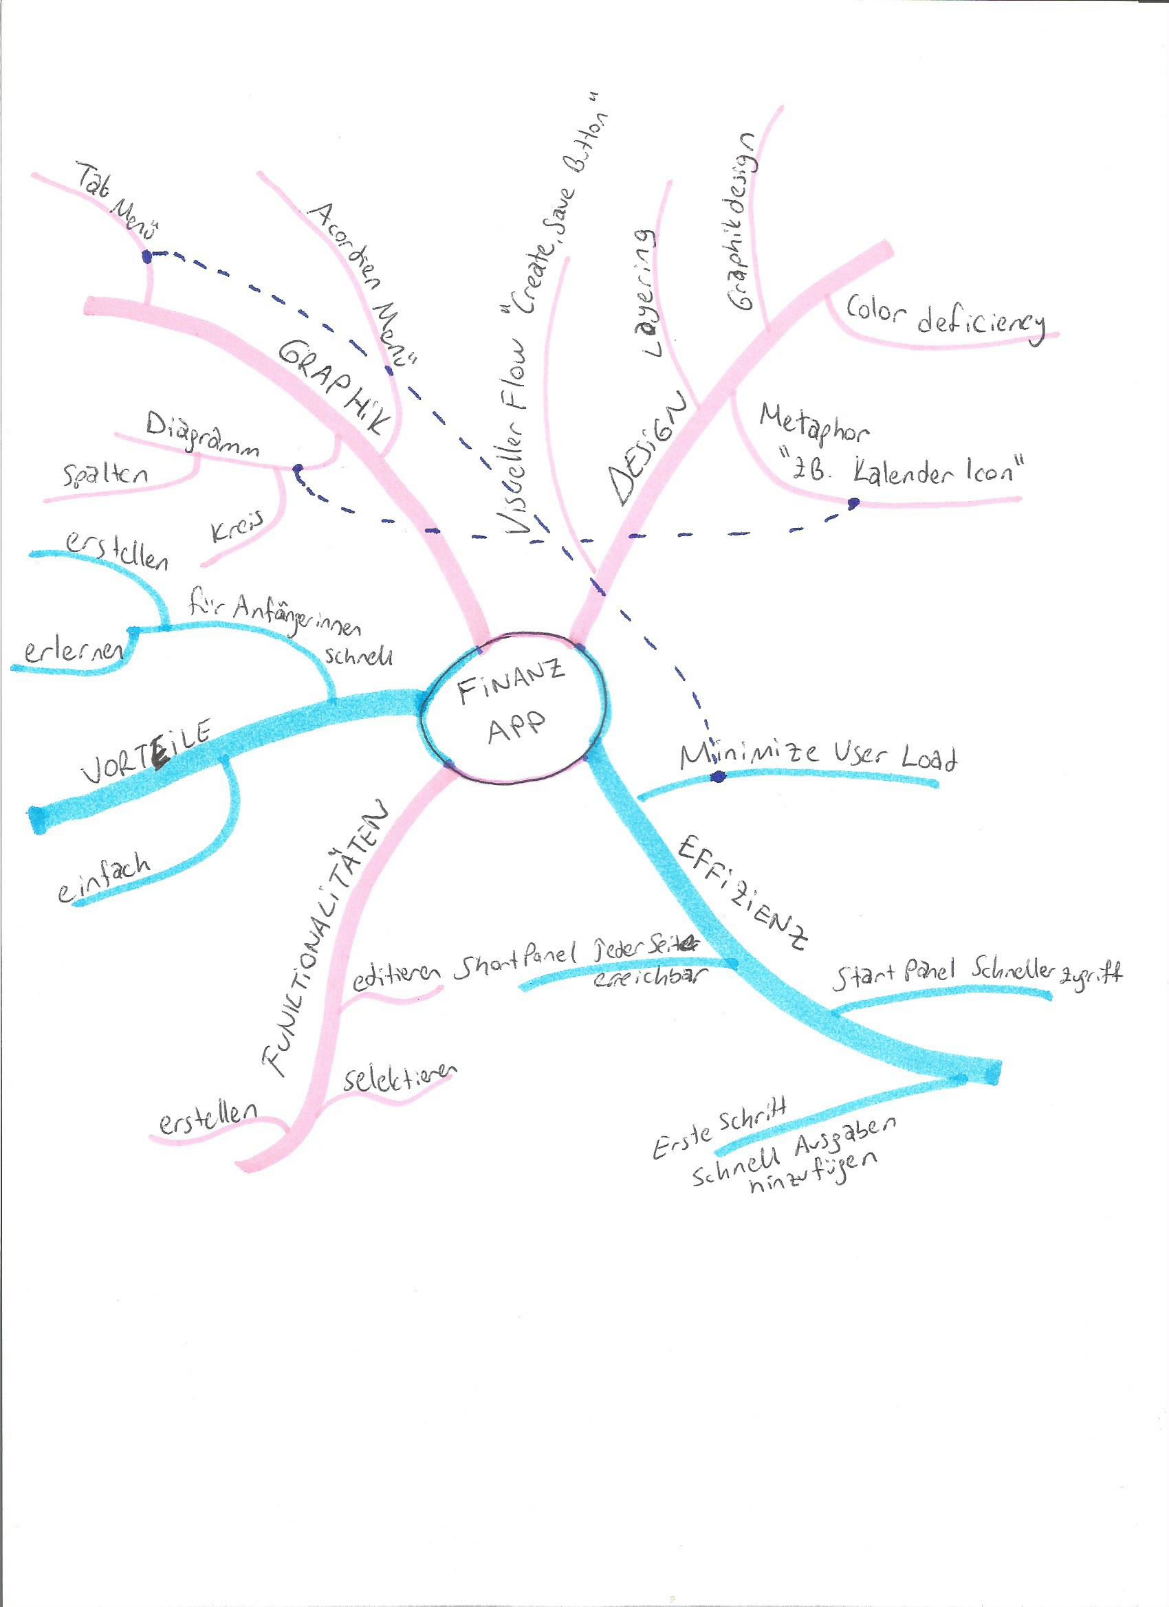
\includegraphics[width=11cm,height=13cm]{mindmap}}
\end{figure}


\clearpage

\section{Low-fi Prototypen}
\subsection{Prototyp-1}

Um die Effizienz zu steigern haben wir uns entschieden als Startseite die "Ausgaben Hinzufügen (Add Expense) " Funktion zu verwenden. Somit kann der User sofort die Hauptfunktion verwenden. 
Unser erster Prototyp listet die entsprechenden Felder welche für eine Ausgabe befüllt werden müssen auf. [a]
Links oben befindet sich ein Shortcut zum Side Panel. Nach einem Touch auf diesen "Bar" wird das seitliche Menü angezeigt [b]. Hier werden alle erreichbaren Menüpunkte aufgelistet. Dieser Side Panel ist von jeder Seite aus erreichbar.
Die "Income" Seite dient zur Speicherung eines neuen Einkommens. [c]\\Das Datum, die Menge und die Herkunft sollen hier durch Eingabe Felder abgefragt und gespeichert werden. Durch einen erneuten Aufruf des Side Panels kann man nun, unter anderem, die Report Seite aufrufen.[d]

\begin{figure}
\centering
\subfigure[Ausgabe hinzufügen]{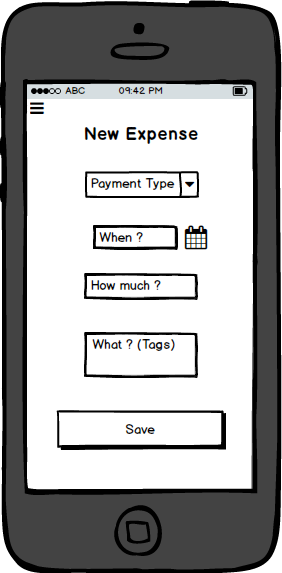
\includegraphics[width=0.20\textwidth]{Expense-1}}
\hfill
\subfigure[Side Panel]{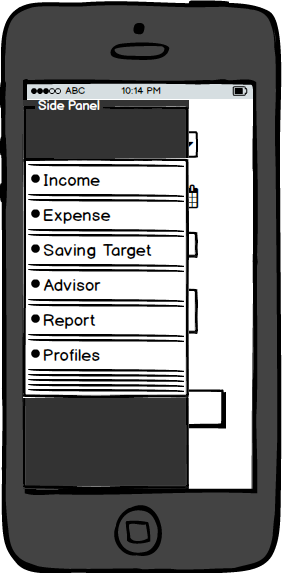
\includegraphics[width=0.20\textwidth]{SidePanel-1}}
\hfill
\subfigure[Enkommen Speichern]{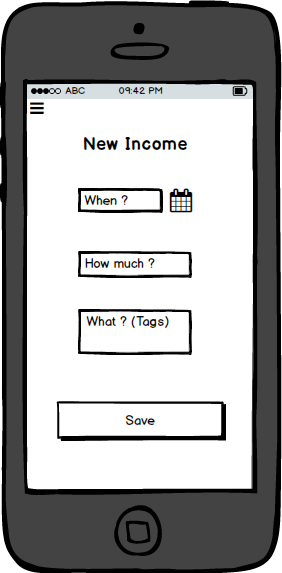
\includegraphics[width=0.20\textwidth]{Income-1}}
\hfill
\subfigure[Bericht erstellen]{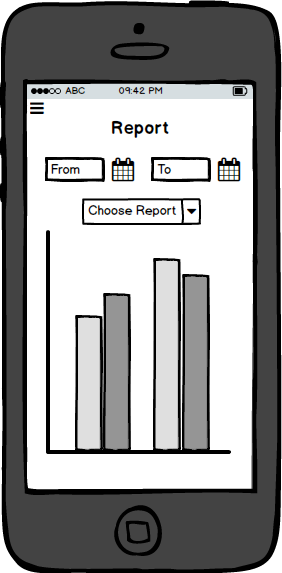
\includegraphics[width=0.20\textwidth]{Report-1}}
\end{figure}



Geplant ist das eine Datumseingabe mittels Start Datum und Enddatum sowie der Typ, durch eine Drop down Auswahl, selektiert werden um somit den entsprechenden Bericht auf der Seite wiederzugeben. Weiteres ist geplant eine Profil Seite zu erstellen [e]. 
Dieser soll durch einen Klick im Side Panel auf dem Menüpunkt "Profiles" erreicht werden.\\ Falls der User noch kein Profil hat kann er nun auf dieser Seite im Drop down Menü "Create New" auswählen welches automatisch auf die Seite "New Profile" weiterleiten wird [f].\\\\ Sollte der User bereits ein Profil haben kann er diesen durch die Auswahl [edit] neben dem Profilenamen im Dropdown die Seite zum Editieren erreichen[g]. Ein Alias für den aktuellen Account, der Name des Users sowie eine Standard Kreditkarten Nummer und die gewünscht Währung soll hier eingegeben werden. Ein weiterer wichtiger Menüpunkt und auch Usecase ist das Sparziel[h] \\Das Ziel dieser Funktion ist es den Nutzern zu ermöglichen Sparziele zu setzten. Diese werden durch die Eingabe des Ziels, das end Datum sowie die Materie selbst festgelegt. Wir planen diese Ziele im Report sowie im Advisor zur berücksichtigen. \\ Obwohl der Advisor nicht zu den primären Usecases gehört, haben wir abschließend trotzdem, um eine Bild vor den Augen zu haben, auch diesen im ersten Prototyp berücksichtigt.[i] \\Wir planen eine Seite die je nach den finanziellen Bewegungen des Users vorgefertigte Ratschläge dynamische erstellt. 


\begin{figure}
\centering
\subfigure[Profile]{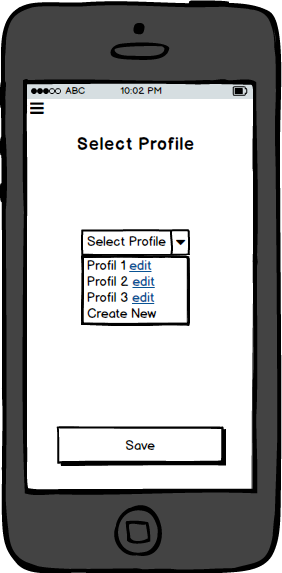
\includegraphics[width=0.20\textwidth]{Profile-1}}
\hfill
\subfigure[Create Profile]{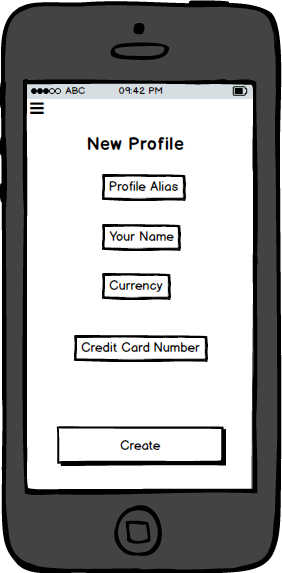
\includegraphics[width=0.20\textwidth]{NewProfile-1}}
\hfill
\subfigure[Edit Profile]{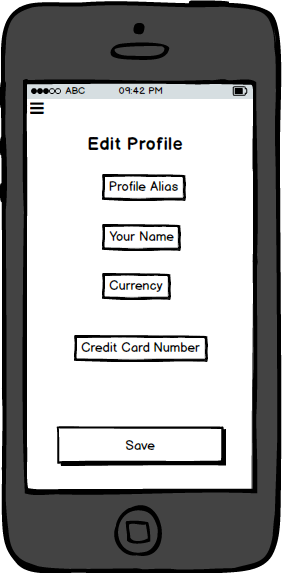
\includegraphics[width=0.20\textwidth]{ChangeProfile-1}}
\vfill
\subfigure[Savetarget erstellen]{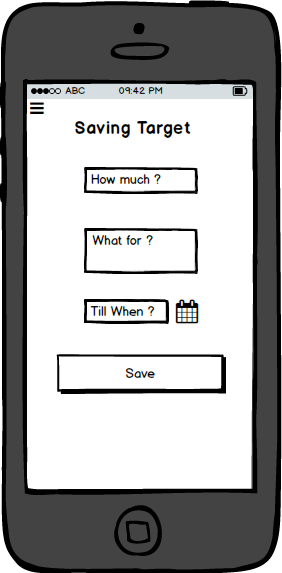
\includegraphics[width=0.20\textwidth]{SavingTarget-1}}
\hfill
\subfigure[Advisor]{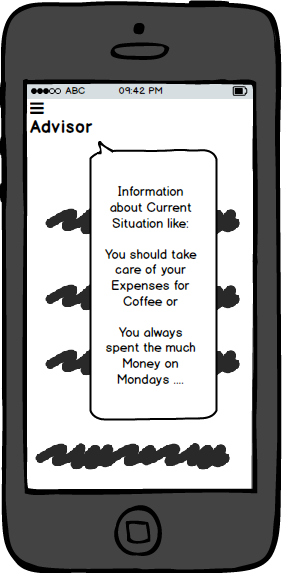
\includegraphics[width=0.20\textwidth]{Advisor-1}}
\end{figure}

\clearpage
\subsection{Prototyp-2}

Der zweite Prototyp unterscheidend sich in Bezug auf den Vorgänger in vielen Punkten. Zur einem haben wir hier den Side Panel abgeschafft und ein Top sowie Bottom Menü eingefügt. Der Vorteil hierbei ist das die punkte stets erreichbar sind und der Nutzer sich das aufklappen des Side Panels ersparen kann. Auch die Fragenstellung, die Anrede selbst, sowie die Eingabe sind freundschaftlicher gestaltet. Hierbei verwenden wir ein Accordion Menü verwendet, welches sich nach Klick auf den jeweiligen Frage aufklappt um entsprechend befüllt zu werden. [j] [k] [l] 

\begin{figure}
\centering
\subfigure[Ausgabe hinzufügen]{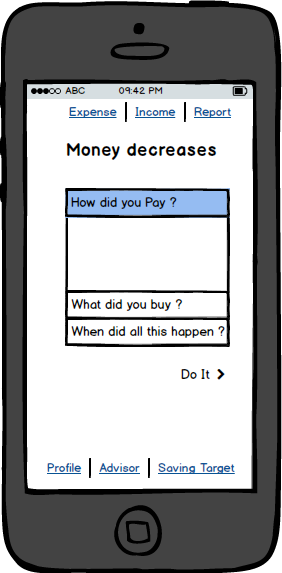
\includegraphics[width=0.15\textwidth]{Expense-2}}
\hfill
\subfigure[Sparziel]{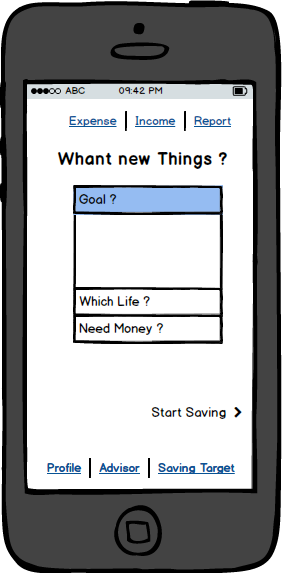
\includegraphics[width=0.15\textwidth]{SavingTarget-2}}
\hfill
\subfigure[Enkommen Speichern]{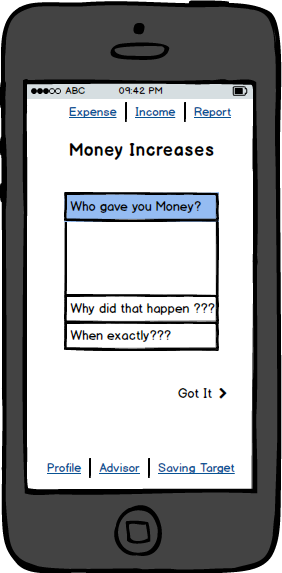
\includegraphics[width=0.15\textwidth]{MoneyIncreases-2}}
\vfill
\subfigure[Select Profil]{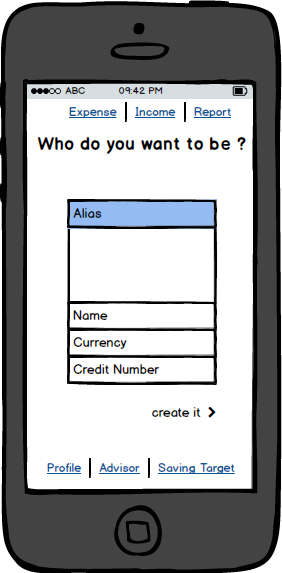
\includegraphics[width=0.15\textwidth]{CreateProfile-2}}
\hfill
\subfigure[Create Profile]{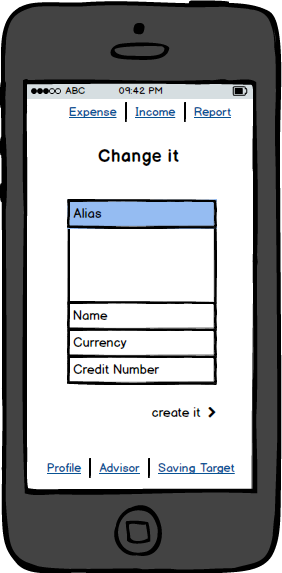
\includegraphics[width=0.15\textwidth]{ChangeProfile-2}}
\hfill
\subfigure[Change Profile]{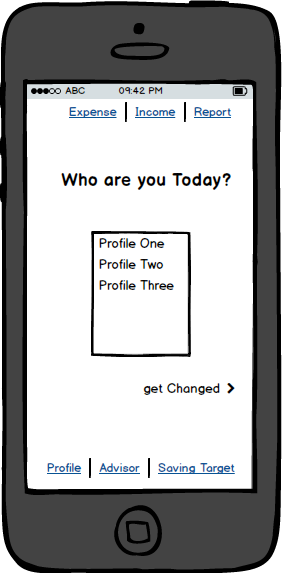
\includegraphics[width=0.15\textwidth]{SelectProfile-2}}
\hfill
\subfigure[Report]{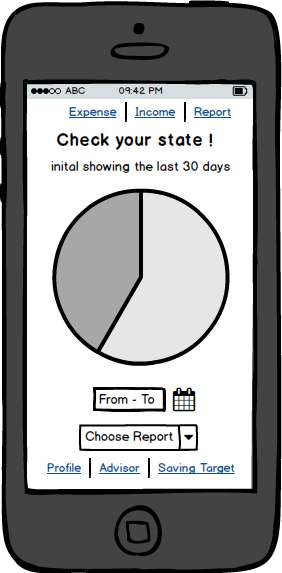
\includegraphics[width=0.15\textwidth]{Report-2}}
\end{figure}

Neben dem freundschaftlichem Touch und auch des Accordion Menüs sind auch die Formulierungen weniger seriös als wie zuvor. Beispiele "Select Profile" [m] oder "Create Profile" [n] bzw. Change Profile [o]. Beim Report haben wir versucht sofort ohne vorherige Abfrage einen initialen Bericht über einen bestimmten Zeitraum zu erstellen. Auch die Datumselektion sollte durch nur einem Feld erleichtert werden. [p]

\clearpage

\subsection{Prototyp-3}

In unserem dritten Prototyp haben wir uns für ein Tab Menü entschieden. Dies sieht zur den beiden Vorgängern zwar etwas überfüllter aus, ist zugleich aber auch strukturierter. [q] Es ermöglicht jedes Feld fast wie eine eigene Seite zu behandeln und würde sehr viel Beschreibung zulassen [r].\\\\ Hierbei haben neben einem horizontalen Tab Menü nämlich auch ein seitlichen Menü eingebaut.[s][t] Der Aktionsbutton (Speichern etc.) befindet sich global im darunter welches die Ansteuerung der Seiten bzw. die Durchführung der Eingaben erleichtern könnte. Dieses Design könnte sich auch bei der Berichterstellung mit einem seitlichen Chart [u] bezahlt machen.\\\\ Die Profile war es bei den Vorgänger notwendig, aufgrund der unterschiedlichen Funktionalitäten (erstellen, selektieren, editieren) eigene Seiten zu erstellen. In diesem Prototyp hat der Nutzer die Möglichkeit, alle relevanten Funktionen, mit nur einem Klick zu erreichen [v]. 

\begin{figure}
\centering
\subfigure[Ausgabe hinzufügen]{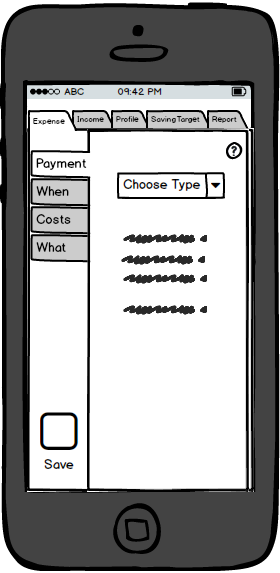
\includegraphics[width=0.15\textwidth]{Expense-3}}
\hfill
\subfigure[Sparziel]{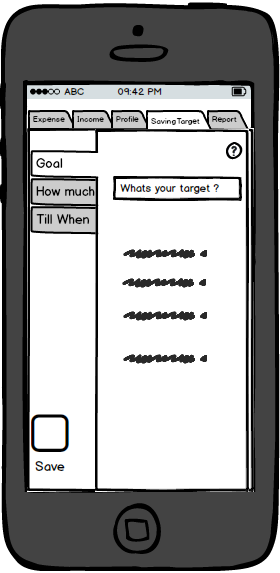
\includegraphics[width=0.15\textwidth]{SaveTarget-3}}
\hfill
\subfigure[Enkommen Speichern]{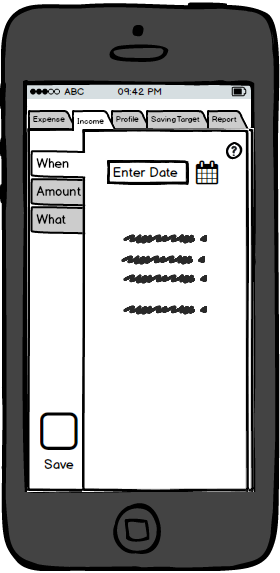
\includegraphics[width=0.15\textwidth]{Income-3}}
\vfill
\subfigure[Change Profile]{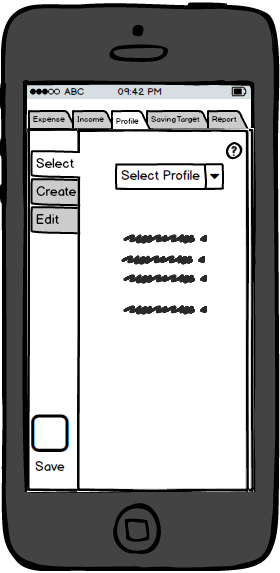
\includegraphics[width=0.15\textwidth]{SelectProfile-3}}
\hfill
\subfigure[Report]{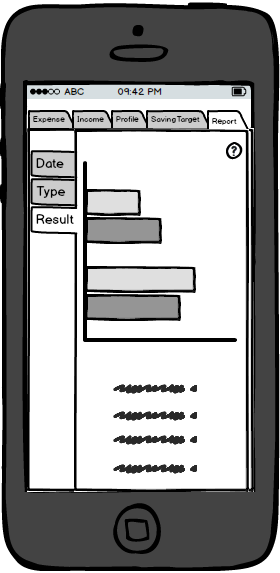
\includegraphics[width=0.15\textwidth]{Report-3}}
\hfill
\subfigure[Select Profil]{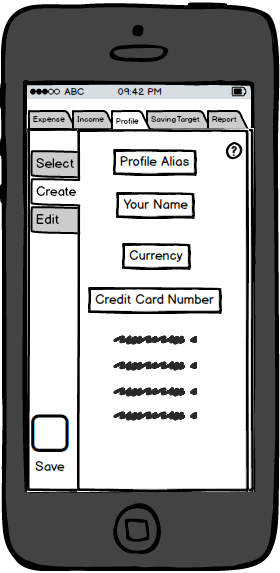
\includegraphics[width=0.15\textwidth]{CreateProfile-3}}
\end{figure}


\clearpage



\section{Interviews}

Evaluierung der Prototypen\\\\
Nach den Phasen der Ideensammlung durch Mindmapping und Erstellung der Prototypen führten wir Interviews mit mehreren Studentinnen und stellten Ihnen unsere drei low fidelity Prototypen vor, um herauszufinden, welche der  drei im Bezug auf Usabilty und Funktionalität die Durchsetzungsstärke besitzt. 
\\
Beschreibung der Interviews hinsichtlich der Vorgehensweise

\begin{figure}
\centering
\subfigure[Flussdiagramm Prototypen-Interview]{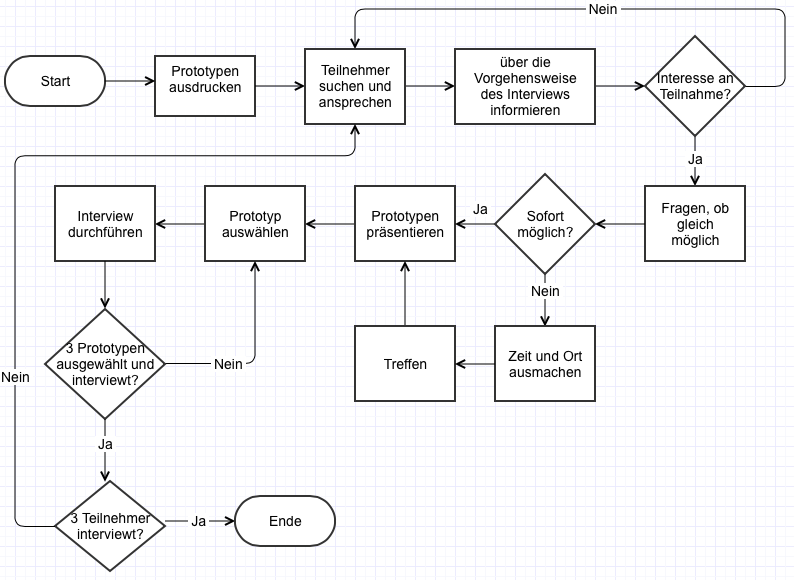
\includegraphics[width=7cm,height=7cm]{flussdiagramInterview}}
\end{figure}


Nachdem wir die drei Prototypen erstellt und auf A4-Papier ausgedruckt haben, haben wir uns auf der Suche nach Teilnehmern für unser Thema begeben. \\Wir suchten uns Studentinnen der Informatik, die wir bereits aus verschiedenen Lehrveranstaltungen kennen  und sprachen sie an.  Wir haben sie über unser Vorhaben, dass wir eine Applikation im Rahmen der Lehrveranstaltung HCI entwickeln, informiert und baten sie zur Beurteilung unserer Prototypen hinsichtlich der Usability und Funktionalität.\\\\ Zwei der drei Studentinnen durften wir gleich dort an der Stelle interviewen. Mit der dritten Person vereinbarten wir am selben Tag einen Termin und trafen uns in einem der Lernräumen der Fakultät Informatik.\\\\
\clearpage
\textbf {Teilnehmer: Onur K. , Stefan B., Bedirhan S.}\\

Die Teilnehmer wurden gebeten, die drei Prototypen genau anzuschauen und uns Ihre Meinung zu äußern. Wir  klärten sie, wie unter Prototypen beschrieben, über die Funktionen, die die geplante Applikation haben soll. Offene Fragen wurden beantwortet.  Im Rahmen der Interviews wurden unter anderem folgende Fragen an die Teilnehmer gestellt.

\begin{itemize}
\item	Welches Prototyp ist für sie leicht zu bedienen?
\item	Welches Prototyp würden Sie hinsichtlich der Usability bevorzugen?
\item	Welche Funktion ist für Sie aus einer Haushaltsbuch-Applikation nicht wegzudenken?
\item	Welches Prototyp gefällt Ihnen am meisten/am wenigsten?
\item	Was hätte man noch besser machen können? Vorschläge?
\end {itemize}

\textbf {Ergebnisse}\\

\textbf {Prototyp 1}: Alle drei Teilnehmer fanden Prototyp 1 leicht zu bedienen und würden sich in der Applikation schnell und einfach zu Recht finden. Side Panel wurde sehr positiv beurteilt, da man dadurch von jedem Untermenü zu dem anderen wechseln kann. \\

\textbf {Prototyp 2}: Das zweite Prototyp kam mit dem Top and Bottom-Menü nicht bei jedem Teilnehmer gut an. Zwei der drei fanden es störend, da man bei jedem Menü sieht und dadurch irritiert werden kann. \\

\textbf {Prototyp 3}: Am wenigsten kam das Prototyp 3 bei den Teilnehmern gut an, da die Schriftgröße im Vergleich viel kleiner war. Alle drei Teilnehmer fanden durch die überfüllten Menüs die schnelle Eintragung der Daten etwas unübersichtlicher.\\

Nach diesen Beurteilungen der Teilnehmern kamen wir zu dem Entschluss, dass wir das Prototyp 1 für unsere Applikation in Betracht ziehen werden. 


\clearpage
\end{document}